\documentclass[a4paper,11pt,oneside,openany]{jsbook}
\usepackage{graphicx,enumerate}
\usepackage{algorithm}
\usepackage{algorithmic}
\usepackage{float}
\usepackage{amssymb}
\usepackage{mathabx}
\usepackage{longtable}
\usepackage{supertabular}
\usepackage{subfigure}

\pagestyle{plain}
\setlength{\textwidth}{\fullwidth}
\setlength{\evensidemargin}{\oddsidemargin}
\def\vector#1{\mbox{\boldmath $#1$}}
\begin{document}
\thispagestyle{empty}
%------------------------------標題紙作成エリア----------------------------%
2015年度 卒業論文%1
\bigskip%2
\LARGE%3
\begin{center}
卒業論文
\end{center}
\bigskip\bigskip\bigskip\bigskip\bigskip\bigskip\bigskip %7
\begin{center} %8
Differential EvolutionにおけるArchiveの性能評価及び改善
\end{center}
\large %11
\begin{center}
Evaluating And Improvement Of Performance Of Archive In Differential Evolution
\end{center}
\bigskip\bigskip\bigskip\bigskip\bigskip\bigskip\bigskip\bigskip\bigskip\bigskip
\bigskip\bigskip\bigskip\bigskip\bigskip\bigskip\bigskip\bigskip\bigskip
\Large %17
\begin{center}
教養学部学際科学科 総合情報学コース
\end{center}
\Large %17
\begin{center}
指導教員: 福永 アレックス
\end{center}
\LARGE %21
\begin{center}
山村 武史
\end{center}
\normalsize
%---------------------------------目次エリア-------------------------------%
\thispagestyle{empty}
\tableofcontents
%---------------------------------本文エリア-------------------------------%

\chapter{序論}  
\section{研究の背景}
実数値最適化問題とは,ある$D$次元の実数値ベクトル$\vector{x} = (x_1, x_2, ..., x_D)$と,それを評価する関数$f(\vector{x})$が与えられたときその評価関数を最小もしくは最大化するような実数値ベクトル$\vector{x}$を探す問題である.
対象問題が,多峰性や悪スケール性,変数分離不可などの特性を有する場合,局所解にトラップされず,大域的な最適解を見つつけだすことが実数値最適化問題において重要となる点の一つである.また多くの実問題については,対象問題が多峰性か,多峰性か,変数分離可か不可かなどといった情報が事前にわからない.このような$\vector{x}$の目的関数値$f(\vector{x})$しかしることが出来ない関数最適化をblack-box optimizationと呼ぶ.
そのような実数値最適化問題を対象とする確率的手法の一つとして,差分進化(Differential Evlolution:DE) \cite{Storn} が用いられる.
最初のDEは,1995年にStornらによって提案された.
DEは処理手順が簡単でありながらも,典型的な実数値GAと比べても最適解に比較的素早く収束する. \cite{Storn} \cite{ExDE}
このためDEは現実的な最適化問題に対して多くの適用例が報告されている \cite{ExDE} .

\section{関連研究}
DEの探索性能は用いる制御パラメタに大きく依存し,そのパラメタは集団数,スケール係数$F$,交叉率$CR$である.しかしこれらのパラメタの適切な値は使用する関数や問題設定によって異なり,実問題をとく上でこれらのパラメタをユーザーが試行錯誤する必要がある.
これらのパラメタを探索中に適応的に変化させていく適応型のDEに関する研究が数多く行われている.
適応型のDE手法としてはJADE \cite{JADE} ,SHADE \cite{SHADE} などが挙げられる.
JADEでは適応戦略以外に,探索性能を強化するために過去の劣解を保持するアーカイブが初めて用いられた.
このアーカイブはJADEにて提唱されその後もSHADEを始めとした多くの適応DEにて使用されている.
しかしアーカイブは問題設定などによっては,探索性能の向上にうまくつながらないこともあり,そのメカニズムについての詳しい研究は未だなされていない.本論文では,アーカイブがDEにおいてどのような役割を果たしているか解明するとともに,従来のアーカイブを改善した手法を幾つか提案する.

\section{本研究の目的}
本研究の目的は2つある.
\begin{enumerate}
\item アーカイブが多様性の維持にどのように役割をはたしているのか調査する
\vspace{3mm}
\newline
アーカイブには,生存選択の時に,劣解として,子個体に上書きされた親個体が保存される.変異ベクトル作成時にアーカイブに保存された劣解を用いることで,解集団における多様性の維持に役立つ.本研究では,アーカイブ使用時と未使用時における解集団の多様性を,目的関数値と,重心からの距離をみることで比較し,解集団が多様性を維持しているかどうか分析を行う.
\newline


\item アーカイブを改良することで,探索性能を向上できないか新たな手法を提案する.
\vspace{3mm}
\newline
アーカイブシステムは多くの適応DEについて使われているにも関わらず,そのシステムについての改良は他の制御パラメタであるスケール係数$F$や交叉率$CR$に比べ試みられていない.
アーカイブ性能の分析をふまえた上で,その改善をはかるための新たな手法を提案する.
\end{enumerate}


\section{本論文の構成}
本論文は以下の通りに構成される。2 章でDEの詳細と適応DE,アーカイブの使用例について説明する.3 章ではアーカイブの性能を重心からの距離と目的関数値$f(\vector{x})$の値をもとに観察する.4章ではアーカイブを改善した手法について説明する.5章では本研究における知見をまとめる.

\chapter{Differential Evolutionとアーカイブ}
\section{Differential Evolution}
まず基本的なDEアルゴリズムについて説明する.DEの集団中の各個体$i \in \{1, ..., N\}$は対象問題の解ベクトル$\vector{x}^i = (x^i_1, ..., x^i_D)$で表現される.ここで$N$は集団数,$D$は次元数である.探索開始時に各個体は探索領域内にランダムに初期化される.その後,突然変異戦略による変異個体の生成,交叉による子個体の生成,生存選択を,探索の終了条件を満たすまで繰り返す.
各世代$t$において各変異個体${\vector{v}^{i,t}}$となる変異ベクトルをその集団中の複数の個体に突然変異戦略を適用することで生成する.代表的な突然変異戦略をTable1にて示す.Table1において${F\in(0,1]}$は突然変異の幅を調整する制御パラメタのひとつスケール係数$F$である.$\vector{x}^{r1},\vector{x}^{r2},\vector{x}^{r3},\vector{x}^{r4},\vector{x}^{r5}$は${\vector{x}^i}$と互いと異なるように集団$\vector{P} = \{ \vector{x}^1, ..., \vector{x}^N \}$からランダムに選択した個体である.$\vector{x}^{best}$は各世代における最良個体であり,$\vector{x}^{pbest}$は集団$P$を評価値の良い順に並び替え,${p\in[0,1]}とした時の上位$max$(N \times p, 2)$個体からランダムに選択した個体である.
current-to-$p$best/1とrand-to-$p$best/1の${\vector{x}^{Ar2}}$,${\vector{x}^{Ar3}}$は集団$P$と後述のアーカイブ$A$の集合からランダムに選択した個体である.
それぞれの突然変異戦略をみていくとbest/1,best/2は変異個体{$\vector{v}^i$}をを最良個体$\vector{x}^{best}$の付近に生成する.
それに対しcurrent-to-best/1は対象個体から$\vector{x}^{best}$にむかうように変異個体{$\vector{v}^i$}を生成する.そのためrand/1やrand/2などに比べ局所的探索能力が強い戦略である.また加える差ベクトルの数が多いほど多様な{$\vector{v}^i$}を生成しやすい.

\begin{table}[htb]
  \begin{center}
  \caption{DEにおける代表的な突然変異戦略}
    \begin{tabular}{ll} \hline
      突然変異戦略 & 定義  \\ \hline
      rand/1 & $\vector{v}_{i} := \vector{x}_{r1} + F\cdot(\vector{x}_{r2} - \vector{x}_{r3})$ \\
      rand/2 & $\vector{v}_{i} := \vector{x}_{r1} + F\cdot(\vector{x}_{r2} - \vector{x}_{r3}) + F\cdot(\vector{x}_{r4} - \vector{x}_{r5})$ \\
      best/1 & $\vector{v}_{i} := \vector{x}_{best} + F\cdot(\vector{x}_{r1} - \vector{x}_{r2})$ \\
      best/2 & $\vector{v}_{i} := \vector{x}_{best} + F\cdot(\vector{x}_{r1} - \vector{x}_{r2}) + F\cdot(\vector{x}_{r3} - \vector{x}_{r4})$ \\
      current-to-rand/1 & $\vector{v}_{i} := \vector{x}_{i} + F\cdot(\vector{x}_{r1} - \vector{x}_{i}) + F\cdot(\vector{x}_{r2} - \vector{x}_{r3})$ \\
      current-to-best/1 & $\vector{v}_{i} := \vector{x}_{i} + F\cdot(\vector{x}_{best} - \vector{x}_{i}) + F\cdot(\vector{x}_{r1} - \vector{x}_{r2})$ \\
      current-to-$p$best/1 & $\vector{v}_{i} := \vector{x}_{i} + F\cdot(\vector{x}_{pbest} - \vector{x}_{i}) + F\cdot(\vector{x}_{r1} - \vector{x}_{Ar2})$ \\
      rand-to-$p$best/1 & $\vector{v}_{i} := \vector{x}_{r1} + F\cdot(\vector{x}_{pbest} - \vector{x}_{r1}) + F\cdot(\vector{x}_{r2} - \vector{x}_{Ar3})$ \\ \hline
    \end{tabular}
  \end{center}
\end{table}


次に親個体$\vector{x}_i$と変異個体$\vector{v}_i$を交叉させることで子個体$\vector{u}_i$を生成する.DEの代表的な交叉手法には二項交叉(binomial crossover)と指数交叉(exponential crossover)がある.以下では二項交叉について紹介する.二項交叉では交叉率$CR \in [0,1]$とランダムに選択した添字$j_{rand} \in \{1,...,D\}$に基づき,Algorithm 1のように子個体$\vector{u}^i = (u^i_1,...,u^i_D)$の各要素$u^i_j$を決定する.

\begin{algorithm}
\caption{二項交叉}
\label{alg:pbnf}
\begin{algorithmic}
\STATE $j_{rand} = \rm{randi}[1, D]$;
\FOR{$j=1$ to $D$}
  \IF {$\rm{rand}[0,1) \leqq $ \OR $j == j_{rand} $}
    \STATE $u^i_j$ := $v^i_j$;
  \ELSE
    \STATE $u^i_j$ := $x^i_j$;
  \ENDIF
\ENDFOR
\end{algorithmic}
\end{algorithm}
全ての個体が子個体を生成した後,次世代に残る個体を決定する.DEでは親個体と子個体の目的関数値を評価関数$f(\vector{x})$を用いて比較し,評価値の良いものを次世代へ残す.
この選択の際,current-to-$p$best/1,及びrand-to-$p$best/1のアーカイブ戦略を用いた場合,子個体より劣っていた親個体$\vector{x}^i$を,アーカイブに保存する.アーカイブのサイズは集団$P$のサイズと等しく,そのサイズを超えた場合,すでにあるアーカイブの中から,ランダムにその要素を取り除く.current-to-$p$best,current-to-randの突然変異戦略において,アーカイブと集団$P$の和集合から親個体$\vector{x}^i$を選択することで,解集団における多様性の維持に役立つ.
最後に本節で述べたDEアルゴリズムの全体をAlgorithm 2に示す.

\begin{algorithm}
\caption{Differential Evolution}
\label{alg:pbnf}
\begin{algorithmic}
\STATE 集団$P={\vector{x}^1,...,\vector{x}^N}$の初期化;
\WHILE {探索終了条件を満たしていない}
    \FOR{$i=1$ to $N$}
        \STATE 突然変異戦略を用いて変異個体{$\vector{v}^i$}を生成;
        \STATE $\vector{x}^i$と$\vector{v}^i$に交叉を適用し,子個体$\vector{u}^i$を生成;
    \ENDFOR
    \FOR{$i=1$ to $N$}
        \IF {$f(\vector{u}^i) \leqq f(\vector{x}^i)$}
            \STATE {$\vector{x}^i :=\vector{u}^i$};
        \ENDIF
    \ENDFOR
\ENDWHILE
\end{algorithmic}
\end{algorithm}


\section{Adaptive Differential Evolution (JADE)}
JADE \cite{JADE} はZhangらによって2009年に提唱された適応型DEの一つである.JADEではDEの探索性能を大きく左右するスケール係数$F$と交叉率$CR$を通常のDEのように固定するのではなく,探索中に自動調整する.その自動調整のために適応メタパラメタ$\mu _F,\mu _{CR}$ を使用する.これらのパラメタは探索開始時に0.5に初期化する.通常のDEでは$F$と$CR$は共通する変数であったが,JADEでは,集団の各個体\vector{x^i}ごとに適応パラメタ$F_i$,$CR_i$を持つ.
そして世代のはじめに$F_i$と$CR_i$を,$\mu _F,\mu _{CR}$をもとにそれぞれ式(2.1),式(2.2)のように更新する.

\begin{eqnarray}
  F_i & = & \rm{randc}(\mu _F, 0.1) \\
  CR_i & = & \rm{randn}(\mu _{CR}, 0.1)
\end{eqnarray}

ここで$\rm{randc}(\mu,\sigma)$は位置パラメタ$\mu$と尺度パラメタ$\sigma$のコーシー分布に従う乱数,$randn(\mu,\sigma^2)$ は平均$\mu$,標準偏差$\sigma^2$の正規分布に従う乱数である.$F_i$の値が$F_i>1$の場合は
$F_i=1$とし $F_i\leqq0$の場合は再び式2.1を用いて生成を行う.$CR_i$の値が区間より外の場合は超えた方の境界値で置き換えられる.
コーシー分布は正規分布に比べ,よりひろがりを持つ分布である.そのためコーシー乱数を使った場合の方が,正規乱数に比べ,多様性を維持したパラメタを生成することが出来る.
各世代の終了後に,成功した${F}$と${CR}$に基づき$\mu_F, \mu_{CR}$を更新する.これらの更新式は式(2.3),式(2.4)となる.

\begin{eqnarray}
  \mu_F & = & (1 - c)\cdot\mu_F + c\cdot mean_L(S_F)\\
  \mu_{CR} & = & (1 - c)\cdot\mu_{CR} + c\cdot mean_A(S_{CR})
\end{eqnarray}

ここで$S_F,S_{CR}$とは,各世代において,生存選択を行う際に親個体よりも優れた変異個体を生成することの出来た$F_i,CR_i$の集合である.次に$c\in[0,1]$は学習率であり推奨値は0.1である.学習率$c$が小さいほど,更新前の$\cdot\mu_F,\cdot\mu_{CR}$に近い値となり,学習率$c$が大きいほど,今の世代で成功した${F}$と${CR}$の値による影響が大きくなる.
また$\rm{mean}_A(\cdot)$は算術平均, $\rm{mean}_L(\cdot)$はLehmer平均でありそれぞれ式(2.5),式(2.6)となる.

\begin{eqnarray}
  mean_A(S) & = \frac{1}{|S|}\sum_{s\in S}s \\
  mean_L(S) & = \frac{\sum_{s\in S}s^2}{\sum_{s\in S}s}
\end{eqnarray}
ここで$S=(s_1,..., s_{|S|})$は$S_F,S_CR$のいずれかである.
JADEのパラメタ適応のメカニズムは,探索中に優れた解を生み出すことの出来たスケーリング係数$F$,交叉率$CR$に近づく形で,それらのパラメタを更新していく.
そのため,理想的なスケーリング係数$F$,交叉率$CR$が,問題設定や探索途中で変わっていくDEにおいて,適切なパラメタを選択することがJADEにおいて可能である.
Algorithm 3はJADEのアルゴリズムの全体である.

\begin{algorithm}
\caption{JADE}
\label{alg:pbnf}
\begin{algorithmic}
\STATE  $\mu_F := 0.5; \mu_{CR} := 0.5f$で初期化;
\WHILE {探索終了条件を満たしていない}
    \STATE $S_F := \emptyset, S_{CR} := \emptyset$;
    \FOR{$i=1$ to $N$}
        \STATE $F_i := \rm{randc}(\mu _F, 0.1)$ \\
        \STATE $CR_i := \rm{randn}(\mu _{CR}, 0.1)$ \\
        \STATE 突然変異戦略を用いて変異個体{$\vector{v}^i$}を生成;
        \STATE $\vector{x}^i$と$\vector{v}^i$に交叉を適用し,子個体$\vector{u}^i$を生成;
    \ENDFOR
    \FOR{$i=1$ to $N$}
        \IF {$f(\vector{u}^i) \leqq f(\vector{x}^i)$}
            \STATE {$\vector{x}^i:=\vector{u}^i$};
            \STATE $S_F := {F_i}, S_CR := {CR_i};$
        \ENDIF
    \ENDFOR
    \IF {$ S_F,S_{CR} \neq \emptyset$}
        \STATE $\mu_F := (1 - c)\cdot\mu _F + c\cdot \rm{mean}_L(S_F)$
        \STATE $\mu_{CR} := (1 - c)\cdot\mu _{CR} + c\cdot  \rm{mean}_A(S_{CR})$
    \ENDIF
\ENDWHILE
\end{algorithmic}
\end{algorithm}

\section{Succes-History based Adaptive Differential Evolution (SHADE)}
さきほどのJADEにつづいて本項では過去の成功したパラメタをもとに適応的にFとCRを変化させるSHADEについて説明する.
JADEでは各世代ごとの成功した有望なパラメタ設定$S_{CR}$, $S_{F}$に近づくようにパラメタを適応させていった.これは$S_{CR}$,$S_F$が対象問題に適したパラメタ値であることを前提としているが,不適切なパラメタ値が$S_{CR}$,$S_F$に含まれる可能性があった.これを防ぐため,SHADEでは大きさ$H$の履歴メモリ$M_F,M_{CR}$を用いてパラメタ適応を行う.これによってJADEに比べ多様なパラメタ値を保持しながら探索を行えるため,よりロバストな探索が可能となっている.
ここで,離散メモリは,$M_F = (M_{F,1},...,M_{F,H})$,$M_{CR}= (M_{CR,1},...,M_{CR,H})$であり,すべての要素は探索開始時に0.5に初期化されている.JADEと同様に集団の各個体\vector{x^i}ごとに適応パラメタ$F_i$,$CR_i$を持ち,これらのパラメータを
各世代のはじめに$[1,H]$の範囲からランダムに選択したメモリの番号$r$の要素$M_{F,r},M_{CR,r}$を用いて式(2.7),式(2.8)のようにして生成する.

\begin{eqnarray}
  F_i & = & \rm{randc}(M_{F,r}, 0.1) \\
  CR_i & = & \rm{randn}(M_{CR,r}, 0.1)
\end{eqnarray}

$F_i$の値が$F_i>1$の場合は$F_i = 1$とし $F_i\leqq1の$の場合は再び式2.7を用いて生成を行う.$CR_i$の値が[0,1]区間より外の場合は超えた方の境界値で置き換えられる.各世代の終了時に成功した$F_i,CR_i$の集合$S_F,S_{CR}$のLehmer平均を用いて,式(2.9),式(2.9)のようにメモリ$M_F,M_CR$を更新する.

\begin{eqnarray}
  M_{F,k} & = & mean_L(S_F)\\
  M_{CR,k} & = & mean_L(S_{CR})
\end{eqnarray}

ここで,$k \in [1,H]$は更新するメモリの要素を決定するパラメタであり,探索開始時に1に初期化され,以降更新を行うたびに1づつ増加していく.また,$k > H$となった場合は$k = 1$とする.探索が経過するに連れて$M_F,M_{CR}$には対象問題に適したかつ,多様なパラメタ設定が保持される.
一つのパラメタ$\mu _F, \mu _{CR}$で管理していたJADEに対し,$M_F = (M_{F,1},...,M_{F,H})$,$M_{CR}= (M_{CR,1},...,M_{CR,H})$とSHADEでは複数のパラメタを持つため,パラメタにおける多様性が維持しやすいのが特徴である.Algorithm 4はSHADEのアルゴリズムの全体である.

\begin{algorithm}
\caption{SHADE}
\label{alg:pbnf}
\begin{algorithmic}
\STATE init all the elements in $M _F$ \& $M _{CR}$ as 0.5;
\STATE k = 1;
\WHILE {the termination crirteria are not met}
    \STATE $S_F := \emptyset, S_{CR} := \emptyset$;
    \FOR{$i=1$ to $N$}
        \STATE $r := \rm{randi}[1,H]$
        \STATE $F_i := \rm{randc}(M_F, 0.1)$ \\
        \STATE $CR_i := \rm{randn}(M_{CR}, 0.1)$ \\
        \STATE 突然変異戦略を用いて変異個体{$\vector{v}^i$}を生成;
        \STATE $\vector{x}^i$と$\vector{v}^i$に交叉を適用し,子個体$\vector{u}^i$を生成;
     \ENDFOR
    \FOR{$i=1$ to $N$}
        \IF {$f(\vector{u}^i) \leqq f(\vector{x}^i)$}
            \STATE {$\vector{x}^i=\vector{u}^i$};
            \STATE $S_F := {F_i}, S_CR := {CR_i};$
        \ENDIF
    \ENDFOR
    \IF {$ S_F,S_{CR} \neq \emptyset$}
        \STATE $M_{F,k}  :=  mean_L(S_F)$;
        \STATE $M_{CR,k}  :=  mean_L(S_{CR})$;
        \STATE $k = (k+1) \% H$;
    \ENDIF
\ENDWHILE
\end{algorithmic}
\end{algorithm} 

\section{DEの探索におけるおける収束性と多様性}
通常のDE及び適応DEについて前節までで説明をした.そしてDEの探索性能は一般的に収束性と多様性の間のバランスを左右するパラメタによって決まる.ここでDEにおける収束性と多様性について再考する.

収束性は,良好な解の近傍に新しい解を発生させることにより,収束性は向上する.DEにおいては,ステップ幅を調整する$F$の値を小さくする.解の更新を速め,子が変位ベクトルに近くなるように$CR$を大きくするなどが.収束性を向上させる.収束性の向上は局所解に陥りやすくなるという欠点がある.

多様性は,広い範囲で新しい解を発生発生させることにより,多様性は向上する.DEにおいては.ステップ幅を調整するFの値を大きくする.解の更新速度を遅くし,急速な収束を差避けるため$CR$を小さくする.アーカイブによる突然変異戦略をとるなどが挙げられる.これによって,大域的な最適解を発見出来る可能性は高くなる代わりに,収束性が低下してしまうという問題がある.

このように収束性と多様性は両者ともトレードオフの関係にあたり,収束性と多様性どちらを優先するかはその探索過程で適応的に変化する必要がある.その収束性と多様性をコントロールするパラメタである$F$と$CR$を探索過程では適応的に変化させるのが前節でのべたJADEやSHADEであった.

次章からは$F$や$CR$のように多様性維持に関わるアーカイブについても,適応的に変化させることでより良い結果が出るようになるのではないか.そもそもアーカイブが多様性の維持に対してどれほど有意な役割をもっているか解析を行う.


\chapter{アーカイブの解析}
\section{アーカイブによる多様性維持の観察}
本章ではアーカイブが解集団における多様性維持に対してどの程度貢献しているかを観察した.実験では解集団における重心からの距離の分散値と,目的関数値関数$f(x)$による分散値をもとに,アーカイブによる多様性の維持について視覚的に観察する.

\section{実験設定}
まず重心からの距離の分散値にもとづきアーカイブの多様性維持について視覚的に観察する.実験では目的関数においてシンプルな関数の一つであるsphere関数を用いて行う.sphere関数は次式で表される短鋒性の関数である.
\begin{eqnarray}
  f(\vector{x}) = \sum_{i=1}^D x_i
\end{eqnarray}

また実行可能領域は$[-100, 100]^D$で次元数$D$は$2,10,30,50,100$,集団数$P$は$10,30,50$,最大試行回数は1試行あたり$D*1,000$とし,試行回数は51回とした.使用したDEは突然変異戦略を式(3.2)のcurrent-to-$p$-best/とし,$F=0.5$,$CR=0.5$である.
$\vector{x}^{r1}$,は${\vector{x}^i}$と異なるように集団$P = {\vector{x}^1, ..., \vector{x}^N}$からランダムに選択した個体であり,また$\vector{x}^{pbest}$は集団$P$を評価値の良い順に並び替え,${p\in[0,1]}$とした時の上位$\rm{max}(N \times p, 2)$個体からランダムに選択した個体である.

\begin{eqnarray}
\vector{v}^{i} = \vector{x}^{i} + F\cdot(\vector{x}^{pbest} - \vector{x}^{i}) + F\cdot(\vector{x}^{r1} - \vector{x}^{Ar2})
\end{eqnarray}

アーカイブありのDEとアーカイブ無しのDEを用いて比較を行う.ここでいうアーカイブありのDEとは式(3.2)における$\vector{x}^{Ar2}$を集団PとアーカイブAの和集合から${\vector{x}^i}$と被らないようにランダムに選択し,アーカイブ無しのDEとは$\vector{x}^{Ar2}$を$x_{i}$と被らないように集団$P$から選択したものである.

多様性を図る尺度としては重心からの距離と目的関数値$f(\vector{x})$の2つの尺度を用いた.
まずある世代$t$の解集団$\vector{P} = \{ \vector{x}^{1,t}, ..., \vector{x}^{N,t} \}$における重心ベクトルを$\vector{x}^{centroid,t}$とする.各$\vector{x}^{k,t}$と重心$\vector{x}^{centroid,t}$の距離$d_{k,t}$を次のように定義する.ただし$k$は$i \in \{1, ..., N\}$となる整数値である.
\begin{eqnarray}
d_{k,t} = \sqrt{\sum_{i=1}^{D} (\vector{x}^{t,centroid,i} - \vector{x}^{t,k,i})^2} 
\end{eqnarray}
$t$世代ごとの集団$P$距離$d_{k,t}$の標準偏差について,51試行の平均値を出すことで多様性を解集団が維持しているかを観察した.
また2つ目の指標として目的関数値$f(\vector{x})$の$t$世代目の集団$P$における標準偏差についても51試行の平均値によって多様性維持の観察を行った.これらの指標が大きな数値を維持出来ているほど,多様性を維持出来ていると考えることができる.


各世代ごとの重心からの距離の標準偏差について,51回の試行の平均値をのせたのが下記一覧である.
表?では目的関数値$f(x)$を用いて,多様性を計測した.ある世代tの解集団$P = {\vector{x}^{t,1}, ..., \vector{x}^{t,N}}$の $\vector{x}^{t,k}$を評価関数であるsphere関数で評価した値$f(s_{t,k})$の標準偏差について,51回の試行の平均値を載せたのが以下の図である.

\section{実験結果}
実験結果をみてみる.図3.1は各世代ごとの重心からの距離の標準偏差,図3.2は各世代ごとの目的関数値による$f(x)$の標準偏差の図である.それぞれ次元数$D$を$2,10,30,50,100$,集団数$P$を$10,30,50$とした時の結果を載せてある.横軸は図3.1,図3.2ともに世代数であり,1~2000世代目までを表示している.
縦軸は,図3.1が各世代$t$の集団$P$における,重心からの距離$d_{k,t}$の標準偏差で,51回試行した平均値に対して常用対数をとったものである.図3.2は各世代$t$の集団$P$における,目的関数値の標準偏差で,51回試行した平均値に対してである.赤色で表示されたデータがアーカイブありのDE,青色で表示されたデータがアーカイブなしのDEとなっている.

これらのデータをまず集団数をもとに見てみる.両者のデータとも集団数が多い時では,アーカイブありのDE,アーカイブなしのDE同士でその多様性の維持に大きな差は見られない.それに対し,集団数が少ない時では,アーカイブありのDE,アーカイブなしのDE同士のデータが世代を経るに連れて,大きくその差を開いている.アーカイブありのDEでは,多様性を維持しているのに対し,アーカイブなしのDEでは,探索が進むに連れて,多様性の維持が難しくなっていることがわかる.

次に次元数を見てみる.両者のデータとも次元数が小さい時では,アーカイブありのDE,アーカイブなしのDE同士でその多様性の維持に大きな差は見られない.それに対し,次元数が大きい時では,アーカイブありのDE,アーカイブなしのDE同士のデータが世代を経るに連れて,その広がりが大きくなっている.これらのことから次元数が大きい時ほど,アーカイブによって集団$P$が多様性を維持しやすくなっていることが伺える.

\begin{figure}[htbp]
  \begin{center}
  \caption{重心からの距離による多様性維持の観察}
    \begin{tabular}{c}


      % 1
      \begin{minipage}{0.33\hsize}
        \begin{center}
          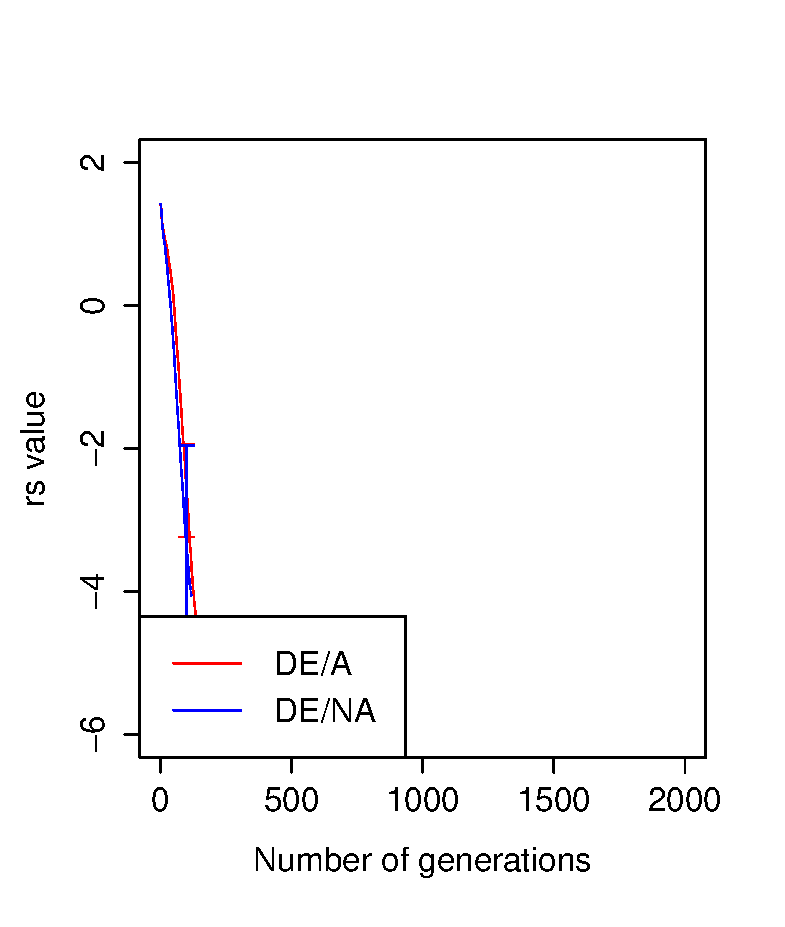
\includegraphics[clip, width=4.0cm]{P10D2.eps}
          \hspace{1.2cm} [1] P=10, D=2
        \end{center}
      \end{minipage}

      % 2
      \begin{minipage}{0.33\hsize}
        \begin{center}
          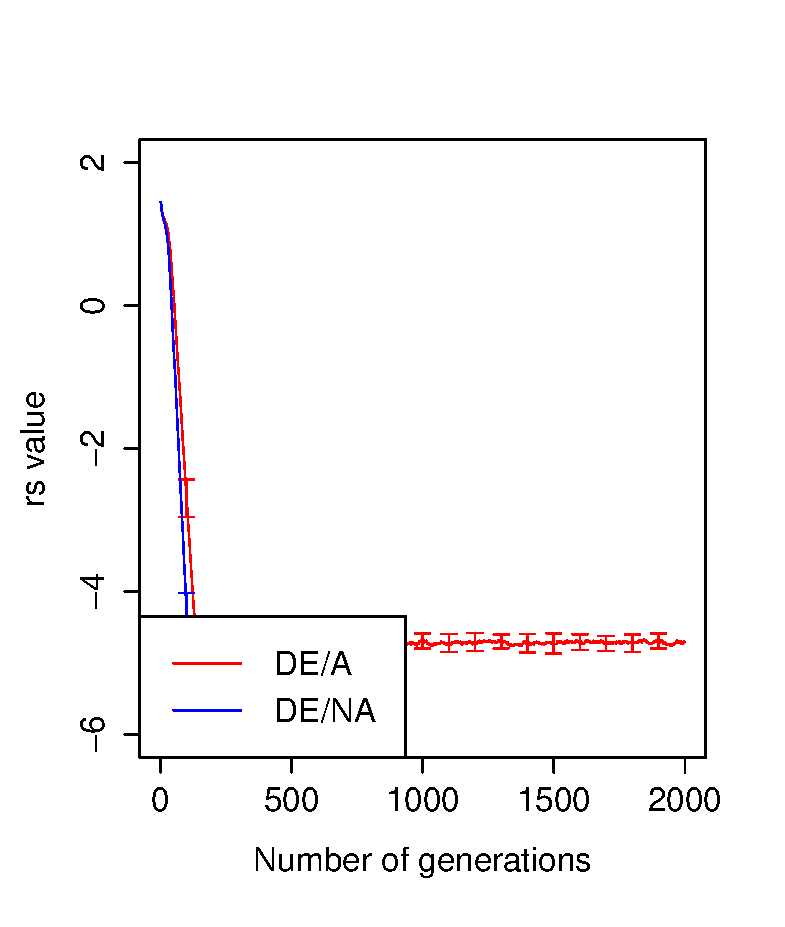
\includegraphics[clip, width=4.0cm]{P30D2.eps}
          \hspace{1.2cm} [2] P=30, D=2
        \end{center}
      \end{minipage}

      % 3
      \begin{minipage}{0.33\hsize}
        \begin{center}
          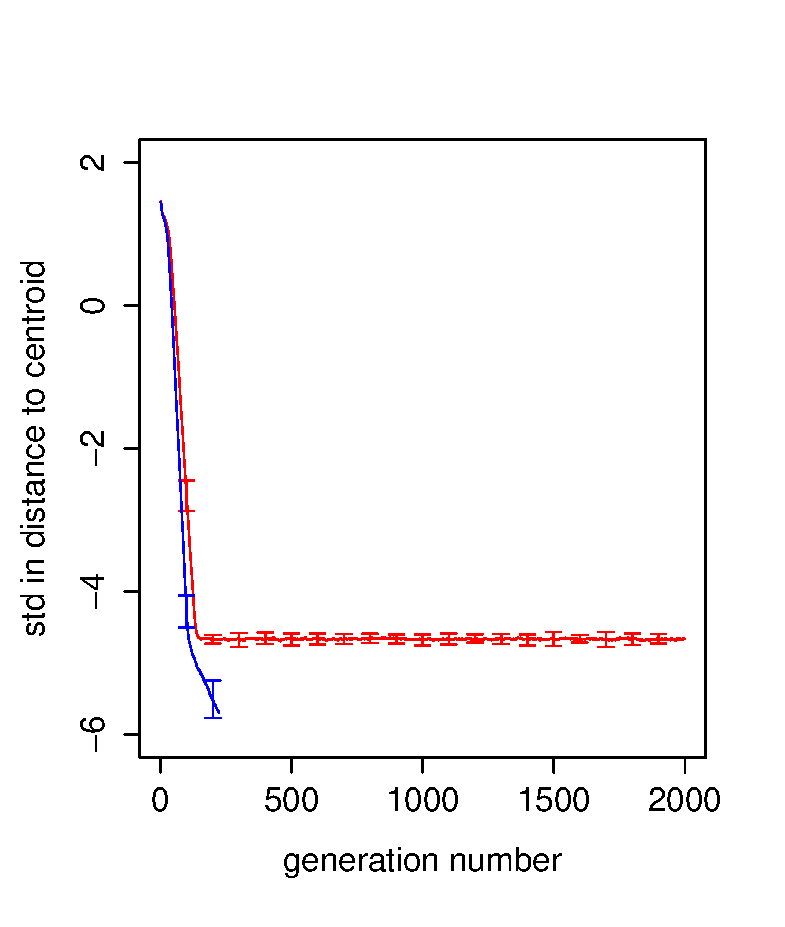
\includegraphics[clip, width=4.0cm]{P50D2.eps}
          \hspace{1.2cm} [3] P=50, D=2
        \end{center}
      \end{minipage}
    \end{tabular}
  \end{center}
\end{figure}
\begin{figure}[htbp]
  \begin{center}
    \begin{tabular}{c}


      % 1
      \begin{minipage}{0.33\hsize}
        \begin{center}
          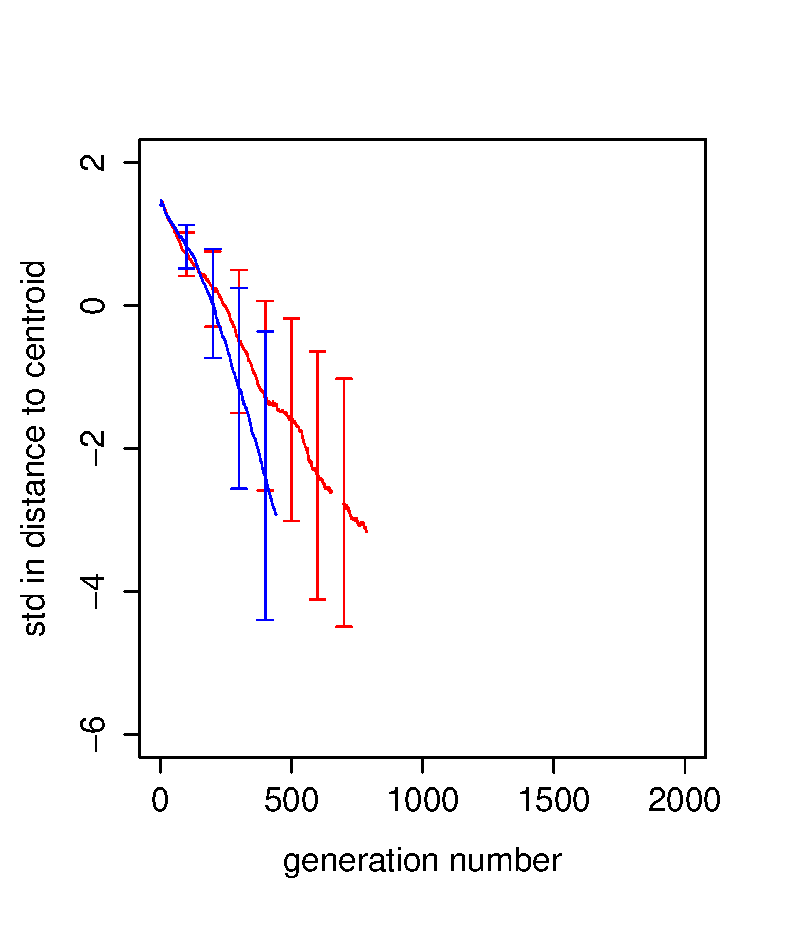
\includegraphics[clip, width=4.0cm]{P10D10.eps}
          \hspace{1.2cm} [4] P=10, D=10
        \end{center}
      \end{minipage}

      % 2
      \begin{minipage}{0.33\hsize}
        \begin{center}
          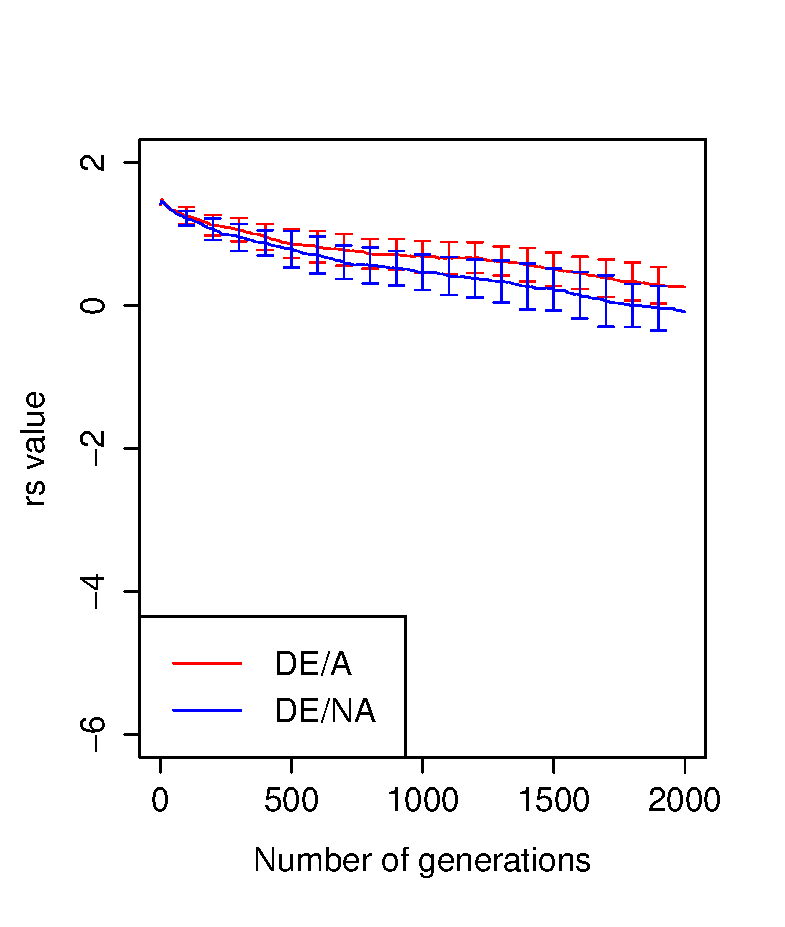
\includegraphics[clip, width=4.0cm]{P30D10.eps}
          \hspace{1.2cm} [5] P=30, D=10
        \end{center}
      \end{minipage}

      % 3
      \begin{minipage}{0.33\hsize}
        \begin{center}
          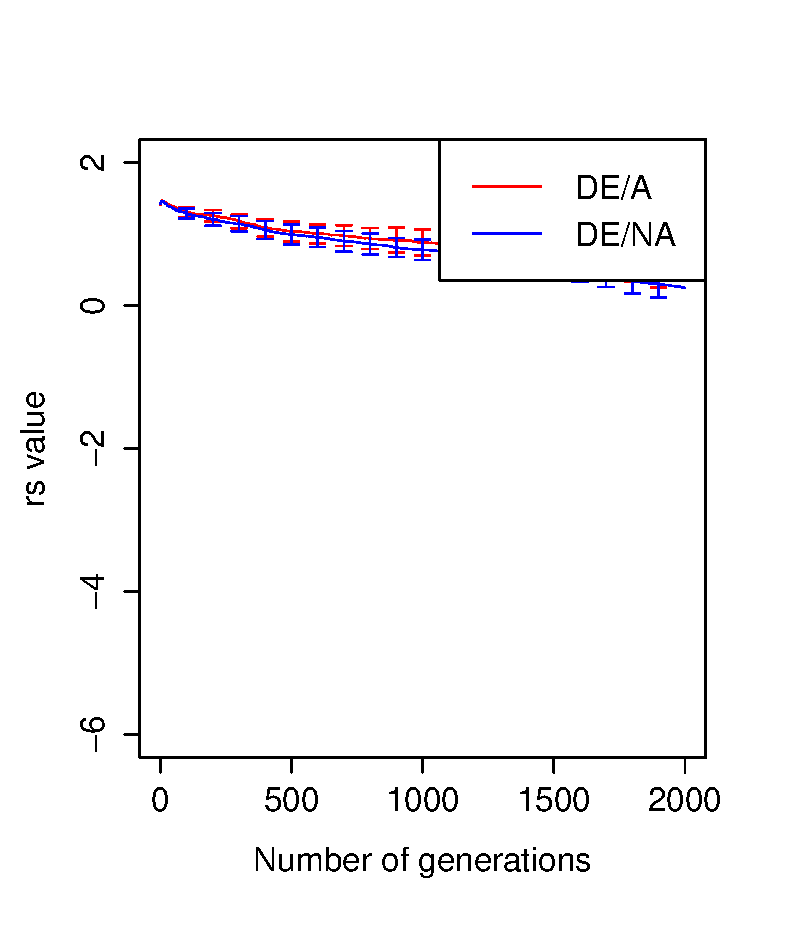
\includegraphics[clip, width=4.0cm]{P50D10.eps}
          \hspace{1.2cm} [6] P=50, D=10
        \end{center}
      \end{minipage}
    \end{tabular}
  \end{center}
\end{figure}
\begin{figure}[htbp]
  \begin{center}
    \begin{tabular}{c}


      % 1
      \begin{minipage}{0.33\hsize}
        \begin{center}
          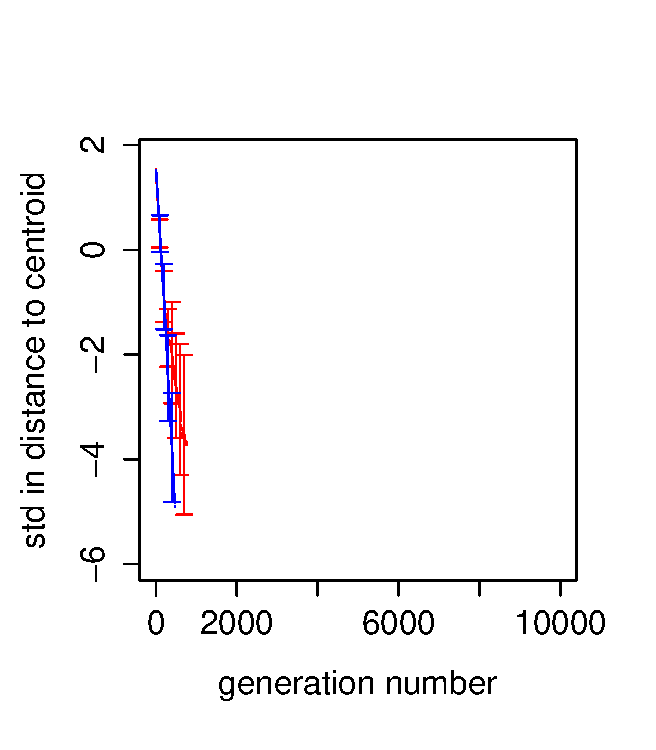
\includegraphics[clip, width=4.0cm]{P10D30.eps}
          \hspace{1.2cm} [7] P=10, D=30
        \end{center}
      \end{minipage}

      % 2
      \begin{minipage}{0.33\hsize}
        \begin{center}
          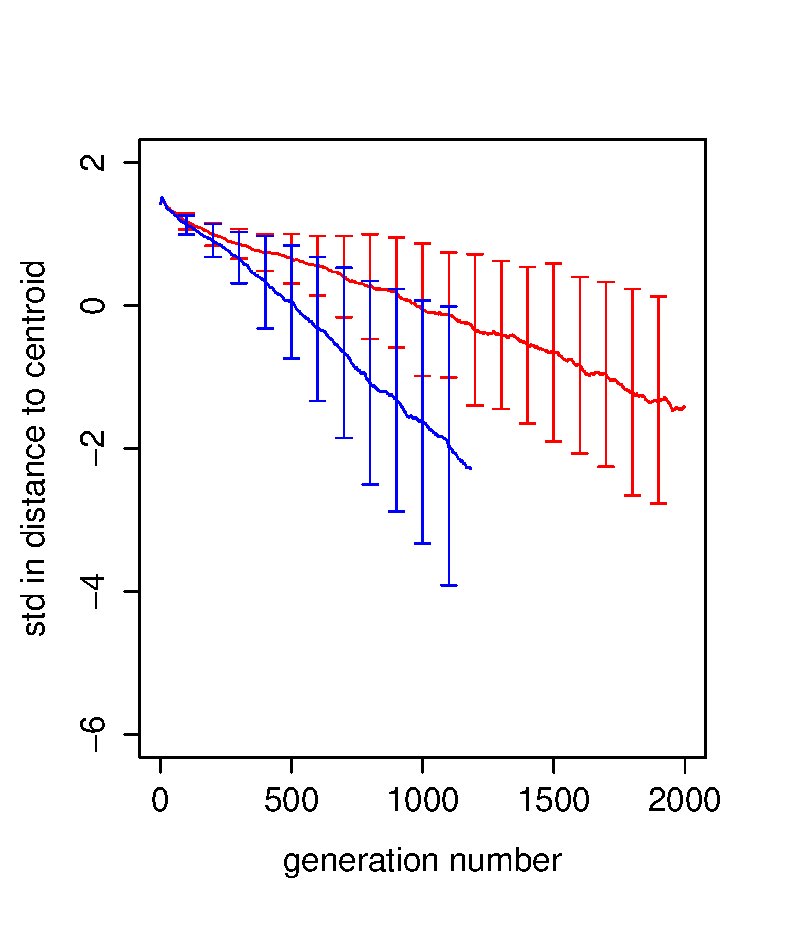
\includegraphics[clip, width=4.0cm]{P30D30.eps}
          \hspace{1.2cm} [8] P=30, D=30
        \end{center}
      \end{minipage}

      % 3
      \begin{minipage}{0.33\hsize}
        \begin{center}
          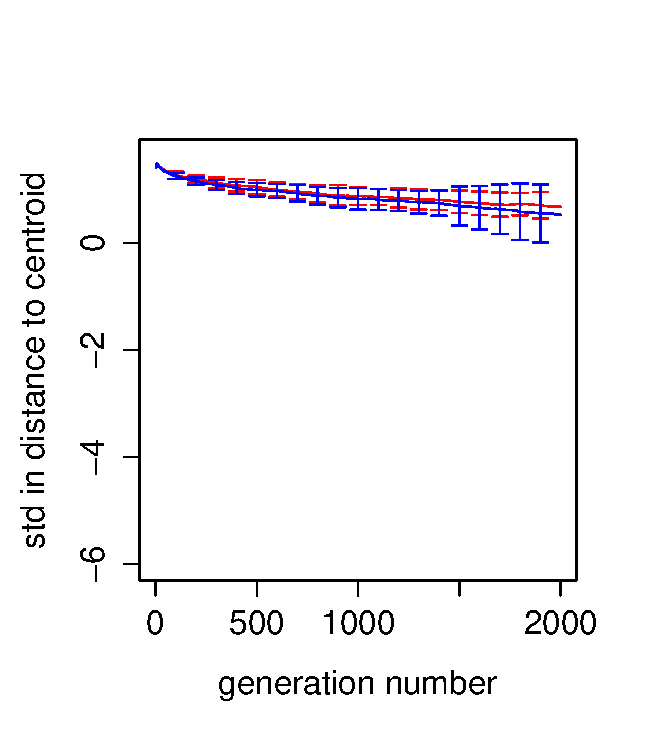
\includegraphics[clip, width=4.0cm]{P50D30.eps}
          \hspace{1.2cm} [9] P=50, D=30
        \end{center}
      \end{minipage}
    \end{tabular}
  \end{center}
\end{figure}
\begin{figure}[htbp]
  \begin{center}
    \begin{tabular}{c}


      % 1
      \begin{minipage}{0.33\hsize}
        \begin{center}
          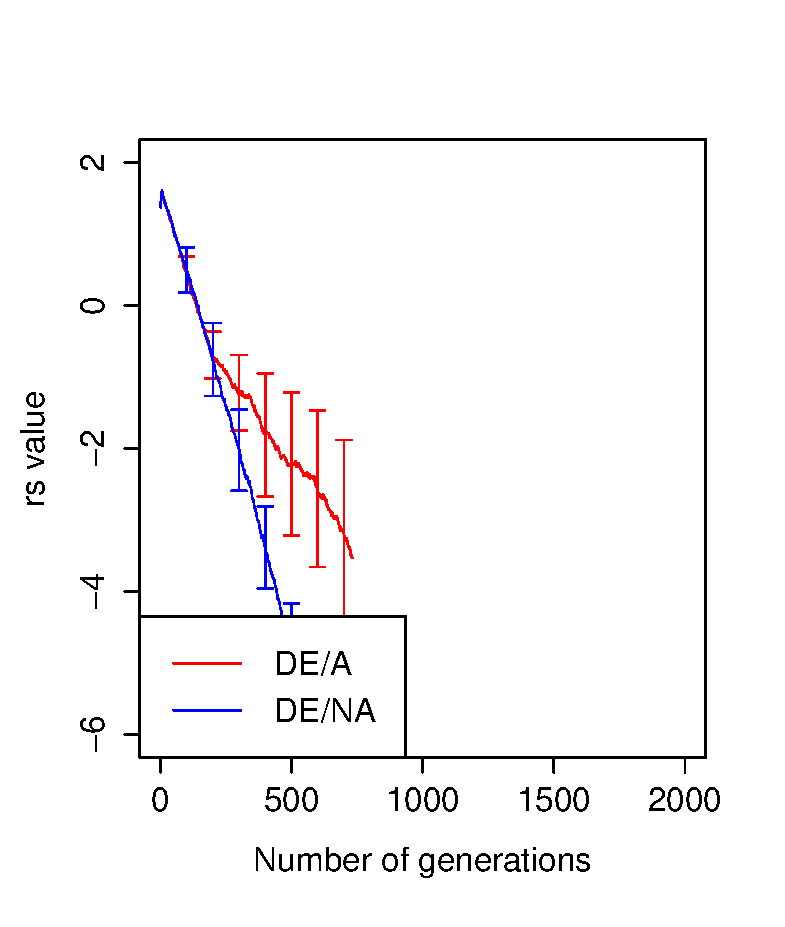
\includegraphics[clip, width=4.0cm]{P10D50.eps}
          \hspace{1.2cm} [10] P=10, D=50
        \end{center}
      \end{minipage}

      % 2
      \begin{minipage}{0.33\hsize}
        \begin{center}
          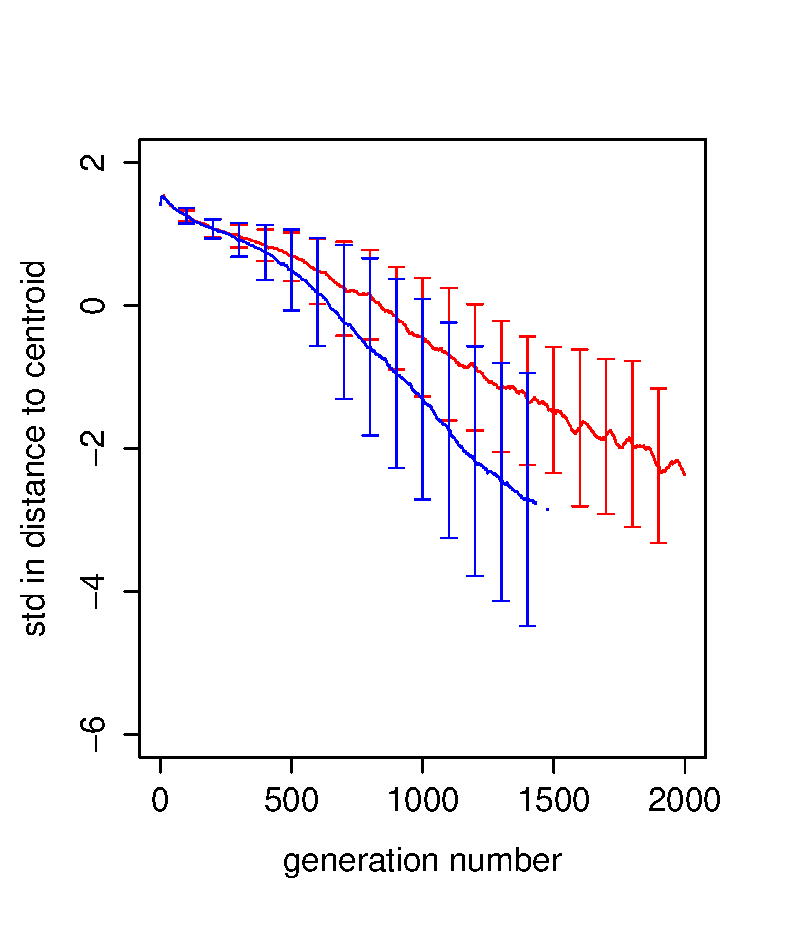
\includegraphics[clip, width=4.0cm]{P30D50.eps}
          \hspace{1.2cm} [11] P=30, D=50
        \end{center}
      \end{minipage}

      % 3
      \begin{minipage}{0.33\hsize}
        \begin{center}
          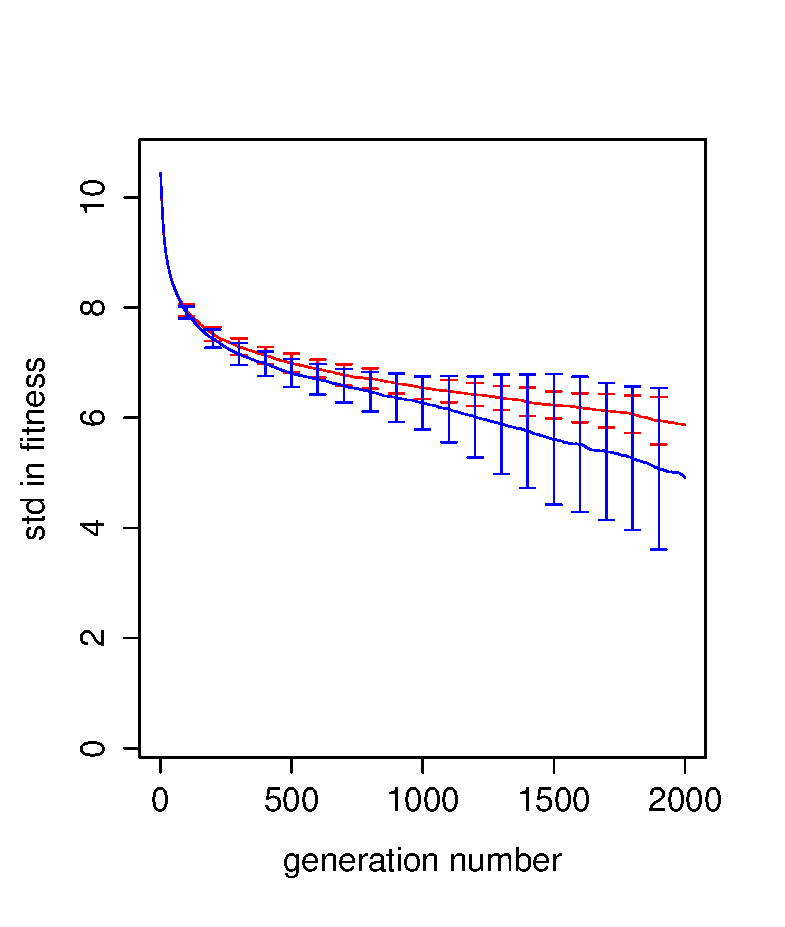
\includegraphics[clip, width=4.0cm]{P50D50.eps}
          \hspace{1.2cm} [12] P=50, D=50
        \end{center}
      \end{minipage}
    \end{tabular}
  \end{center}
\end{figure}
\begin{figure}[htbp]
  \begin{center}
    \begin{tabular}{c}


      % 1
      \begin{minipage}{0.33\hsize}
        \begin{center}
          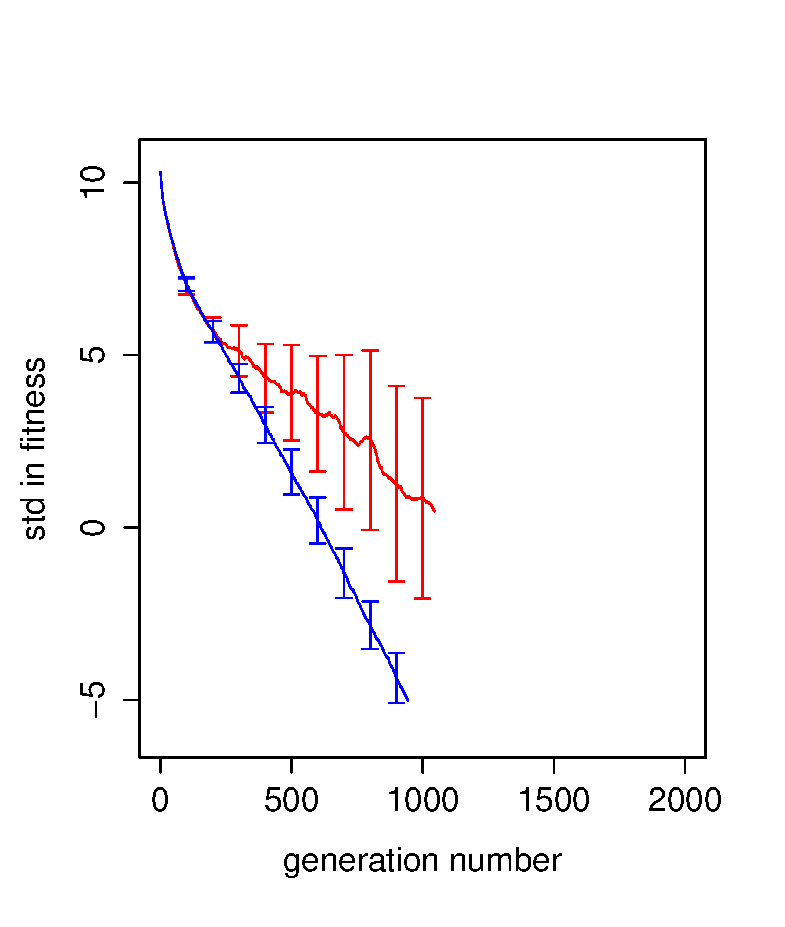
\includegraphics[clip, width=4.0cm]{P10D100.eps}
          \hspace{1.2cm} [13] P=10, D=100
        \end{center}
      \end{minipage}

      % 2
      \begin{minipage}{0.33\hsize}
        \begin{center}
          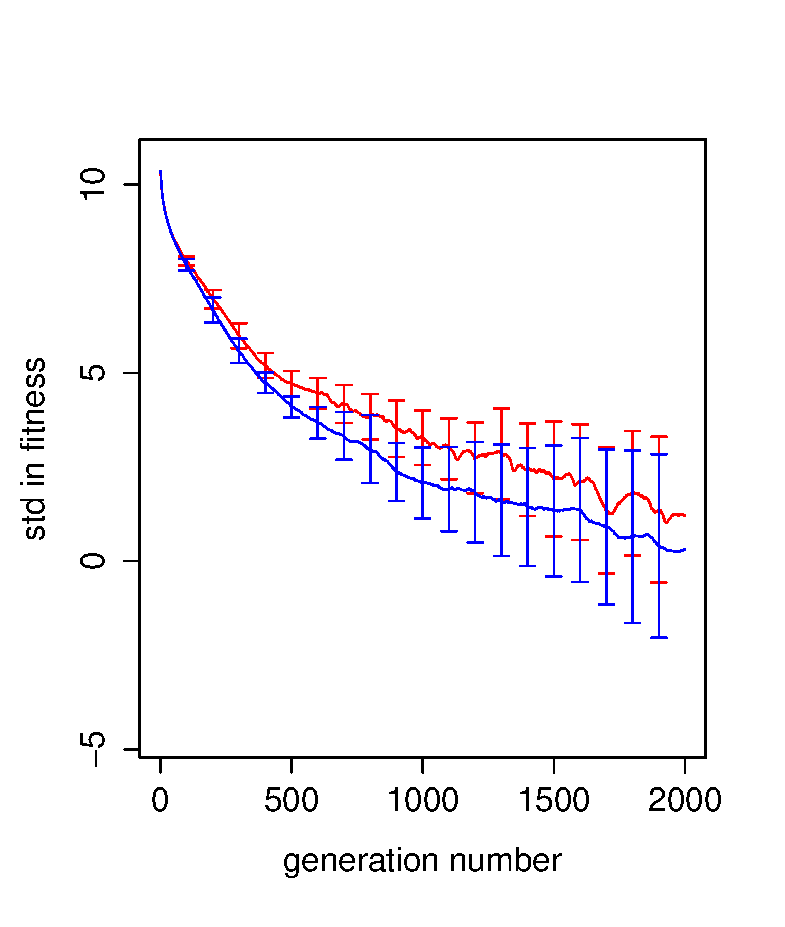
\includegraphics[clip, width=4.0cm]{P30D100.eps}
          \hspace{1.2cm} [14] P=30, D=100
        \end{center}
      \end{minipage}

      % 3
      \begin{minipage}{0.33\hsize}
        \begin{center}
          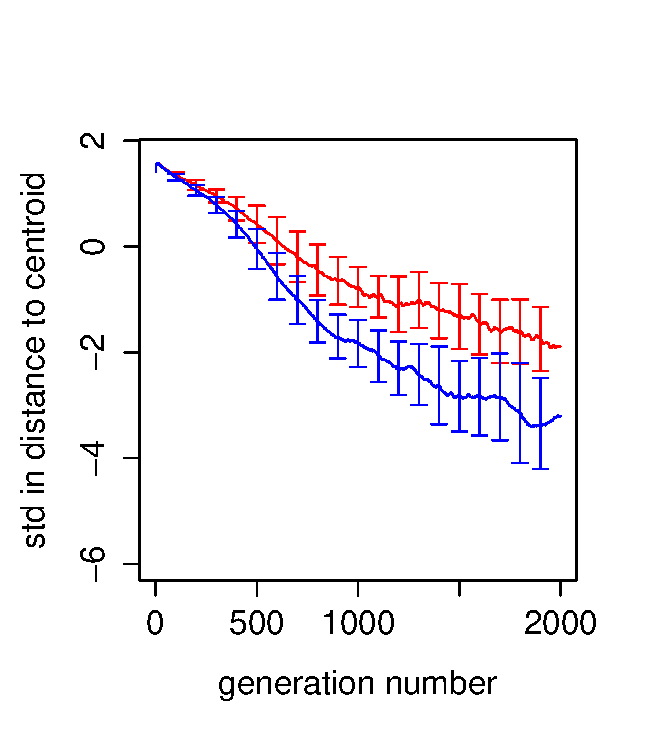
\includegraphics[clip, width=4.0cm]{P50D100.eps}
          \hspace{1.2cm} [15] P=50, D=100
        \end{center}
      \end{minipage}
    \end{tabular}
    \label{fig:lena}
  \end{center}
\end{figure}

% \caption{目的関数値による多様性維持の観察}
\begin{figure}[htbp]
  \begin{center}
  \caption{目的関数値による多様性維持の観察}
    \begin{tabular}{c}


      % 1
      \begin{minipage}{0.33\hsize}
        \begin{center}
          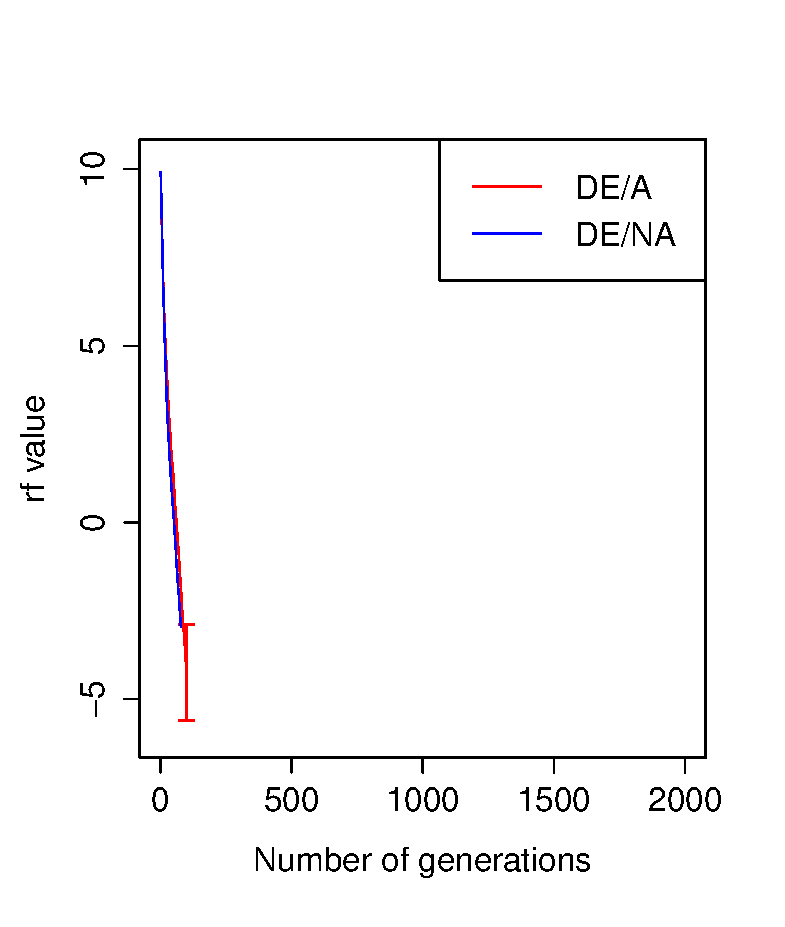
\includegraphics[clip, width=4.0cm]{P10fitD2.eps}
          \hspace{1.2cm} [1] P=10, D=2
        \end{center}
      \end{minipage}

      % 2
      \begin{minipage}{0.33\hsize}
        \begin{center}
          \includegraphics[clip, width=4.0cm]{P30fitD2.eps}
          \hspace{1.2cm} [2] P=30, D=2
        \end{center}
      \end{minipage}

      % 3
      \begin{minipage}{0.33\hsize}
        \begin{center}
          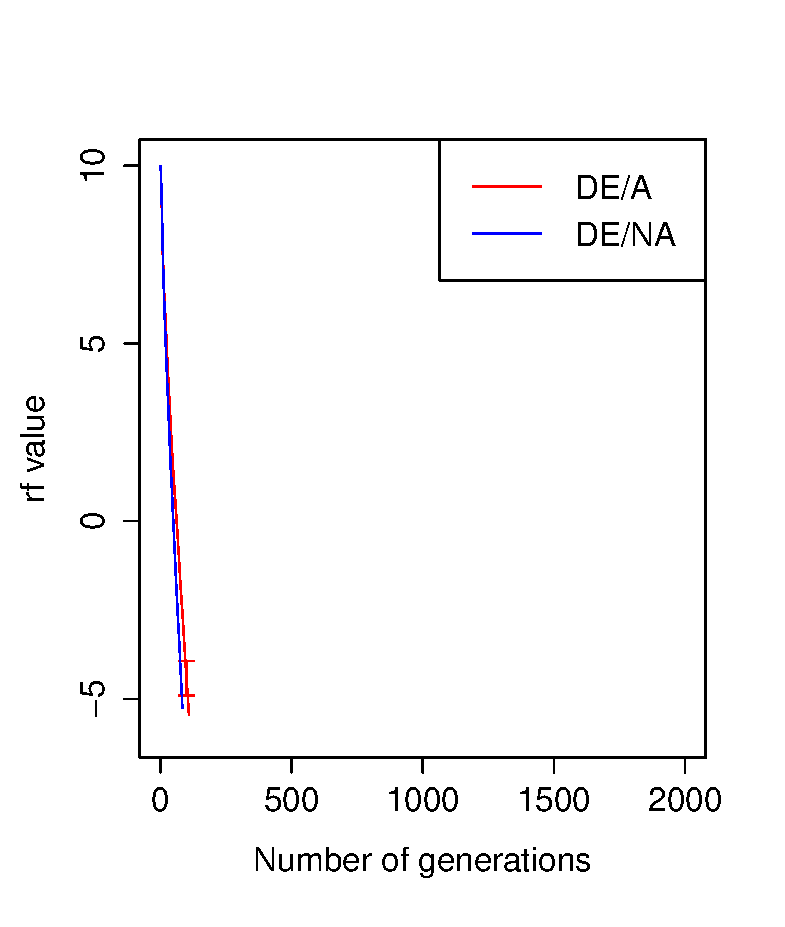
\includegraphics[clip, width=4.0cm]{P50fitD2.eps}
          \hspace{1.2cm} [3] P=50, D=2
        \end{center}
      \end{minipage}
    \end{tabular}
  \end{center}
\end{figure}
\begin{figure}[htbp]
  \begin{center}
    \begin{tabular}{c}


      % 1
      \begin{minipage}{0.33\hsize}
        \begin{center}
          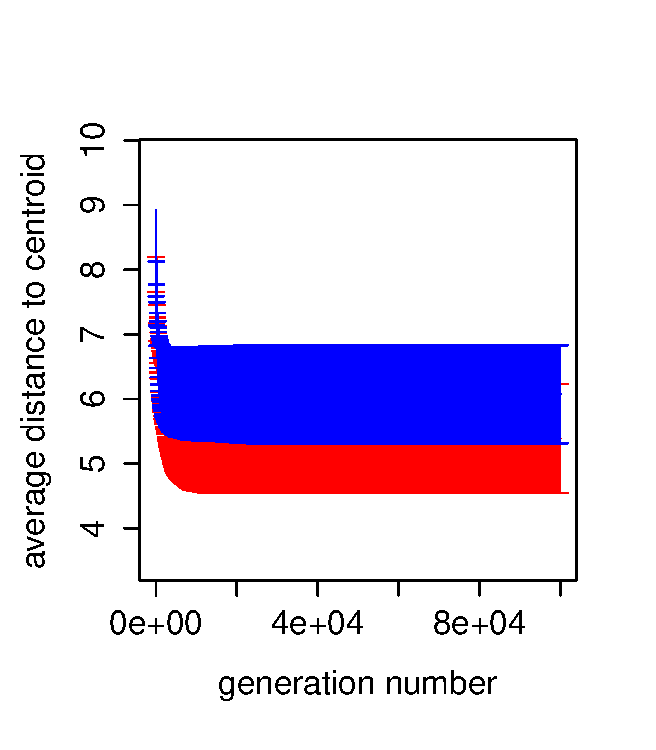
\includegraphics[clip, width=4.0cm]{P10fitD10.eps}
          \hspace{1.2cm} [4] P=10, D=10
        \end{center}
      \end{minipage}

      % 2
      \begin{minipage}{0.33\hsize}
        \begin{center}
          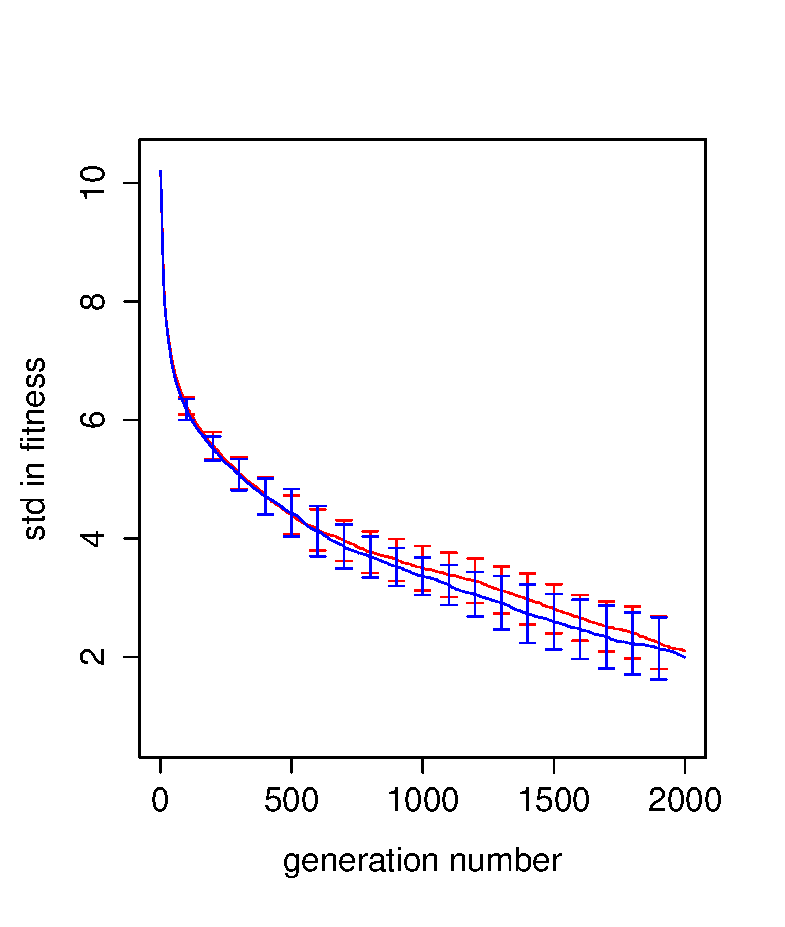
\includegraphics[clip, width=4.0cm]{P30fitD10.eps}
          \hspace{1.2cm} [5] P=30, D=10
        \end{center}
      \end{minipage}

      % 3
      \begin{minipage}{0.33\hsize}
        \begin{center}
          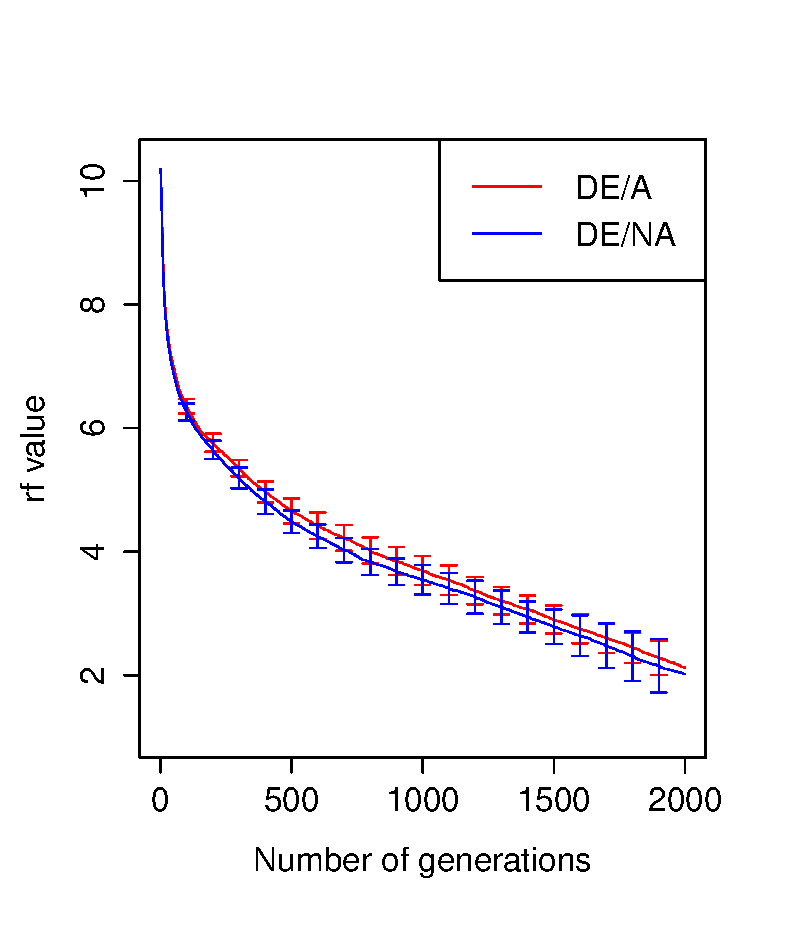
\includegraphics[clip, width=4.0cm]{P50fitD10.eps}
          \hspace{1.2cm} [6] P=50, D=10
        \end{center}
      \end{minipage}
    \end{tabular}
  \end{center}
\end{figure}
\begin{figure}[htbp]
  \begin{center}
    \begin{tabular}{c}


      % 1
      \begin{minipage}{0.33\hsize}
        \begin{center}
          \includegraphics[clip, width=4.0cm]{P10fitD30.eps}
          \hspace{1.2cm} [7] P=10, D=30
        \end{center}
      \end{minipage}

      % 2
      \begin{minipage}{0.33\hsize}
        \begin{center}
          \includegraphics[clip, width=4.0cm]{P30fitD30.eps}
          \hspace{1.2cm} [8] P=30, D=30
        \end{center}
      \end{minipage}

      % 3
      \begin{minipage}{0.33\hsize}
        \begin{center}
          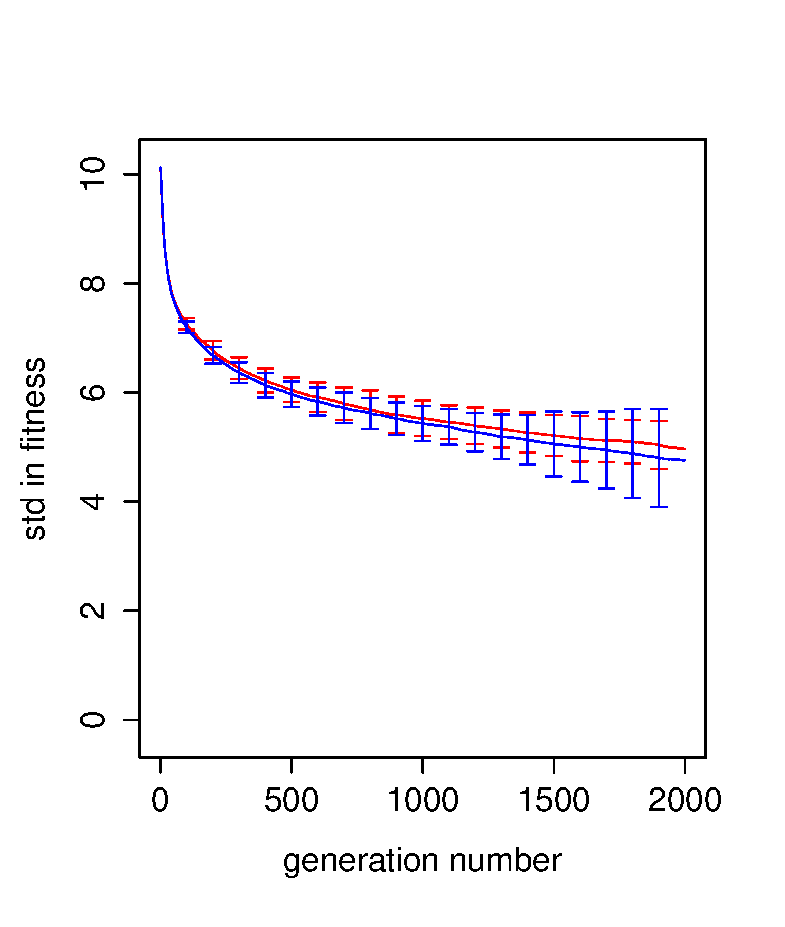
\includegraphics[clip, width=4.0cm]{P50fitD30.eps}
          \hspace{1.2cm} [9] P=50, D=30
        \end{center}
      \end{minipage}
    \end{tabular}
  \end{center}
\end{figure}
\begin{figure}[htbp]
  \begin{center}
    \begin{tabular}{c}


      % 1
      \begin{minipage}{0.33\hsize}
        \begin{center}
          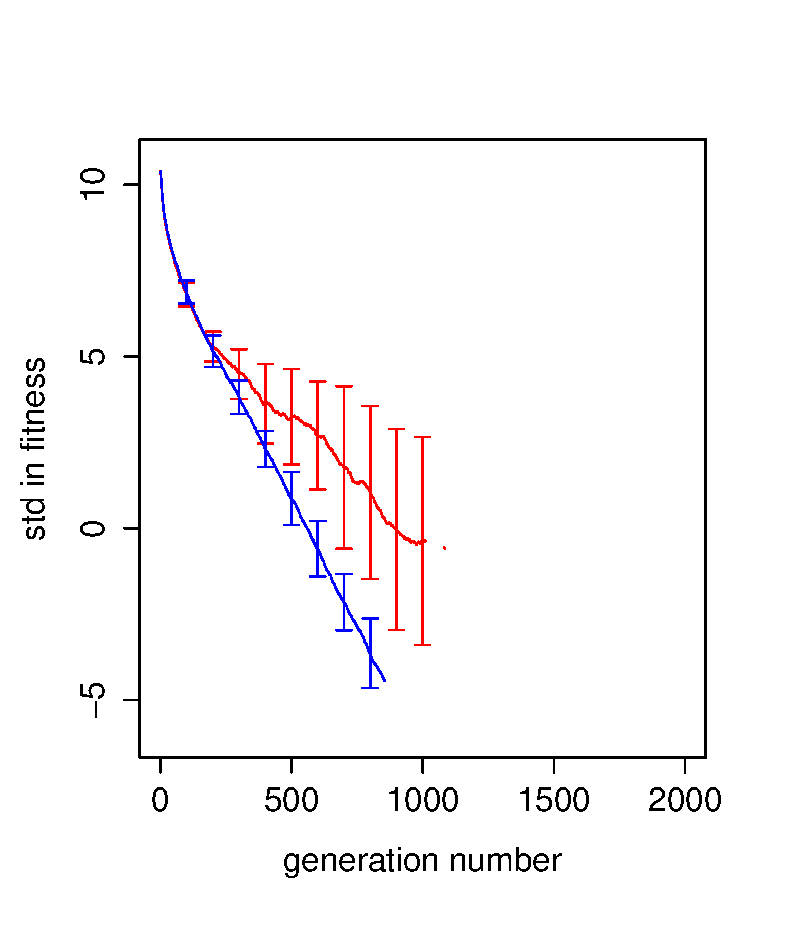
\includegraphics[clip, width=4.0cm]{P10fitD50.eps}
          \hspace{1.2cm} [10] P=10, D=50
        \end{center}
      \end{minipage}

      % 2
      \begin{minipage}{0.33\hsize}
        \begin{center}
          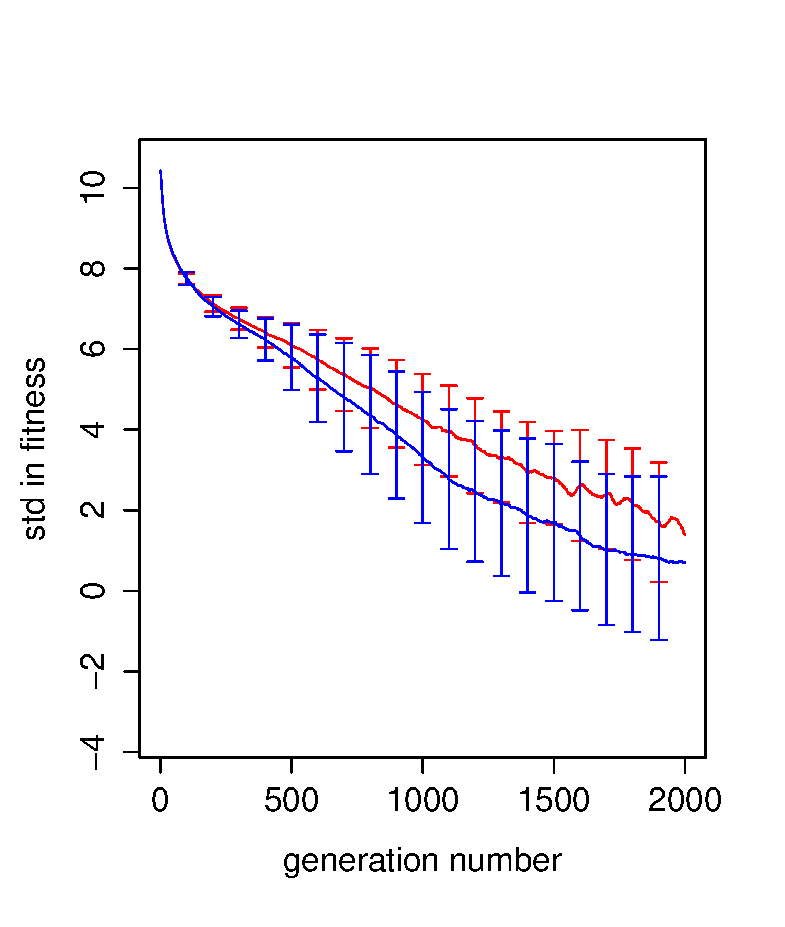
\includegraphics[clip, width=4.0cm]{P30fitD50.eps}
          \hspace{1.2cm} [11] P=30, D=50
        \end{center}
      \end{minipage}

      % 3
      \begin{minipage}{0.33\hsize}
        \begin{center}
          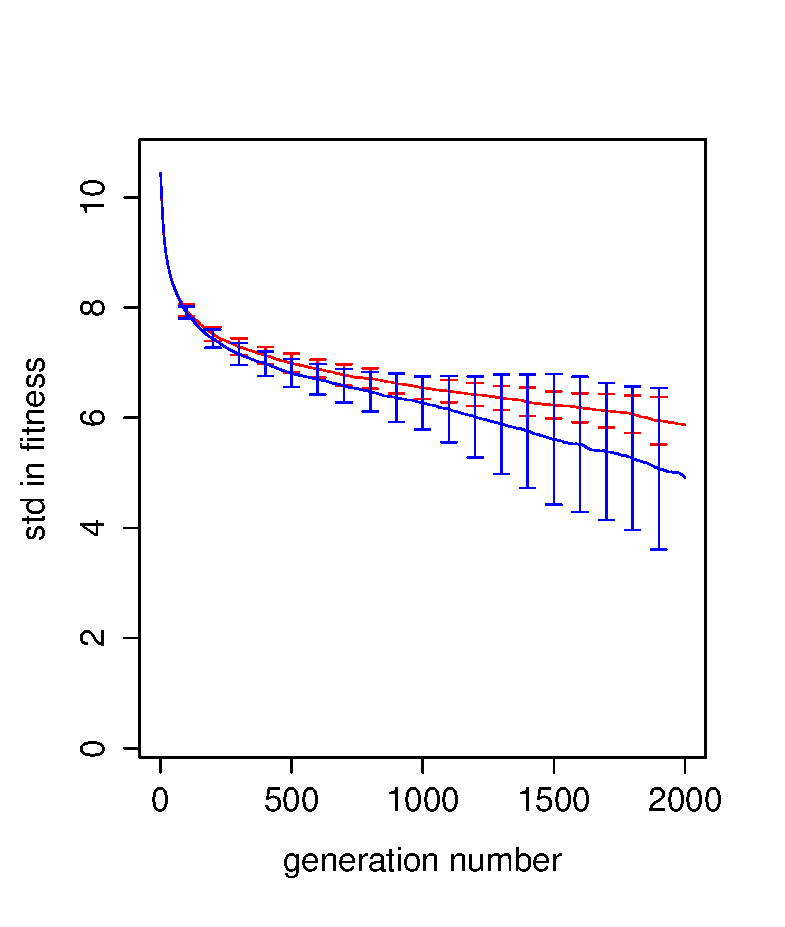
\includegraphics[clip, width=4.0cm]{P50fitD50.eps}
          \hspace{1.2cm} [12] P=50, D=50
        \end{center}
      \end{minipage}
    \end{tabular}
  \end{center}
\end{figure}
\begin{figure}[htbp]
  \begin{center}
    \begin{tabular}{c}

      % 1
      \begin{minipage}{0.33\hsize}
        \begin{center}
          \includegraphics[clip, width=4.0cm]{P10fitD100.eps}
          \hspace{1.2cm} [13] P=10, D=100
        \end{center}
      \end{minipage}

      % 2
      \begin{minipage}{0.33\hsize}
        \begin{center}
          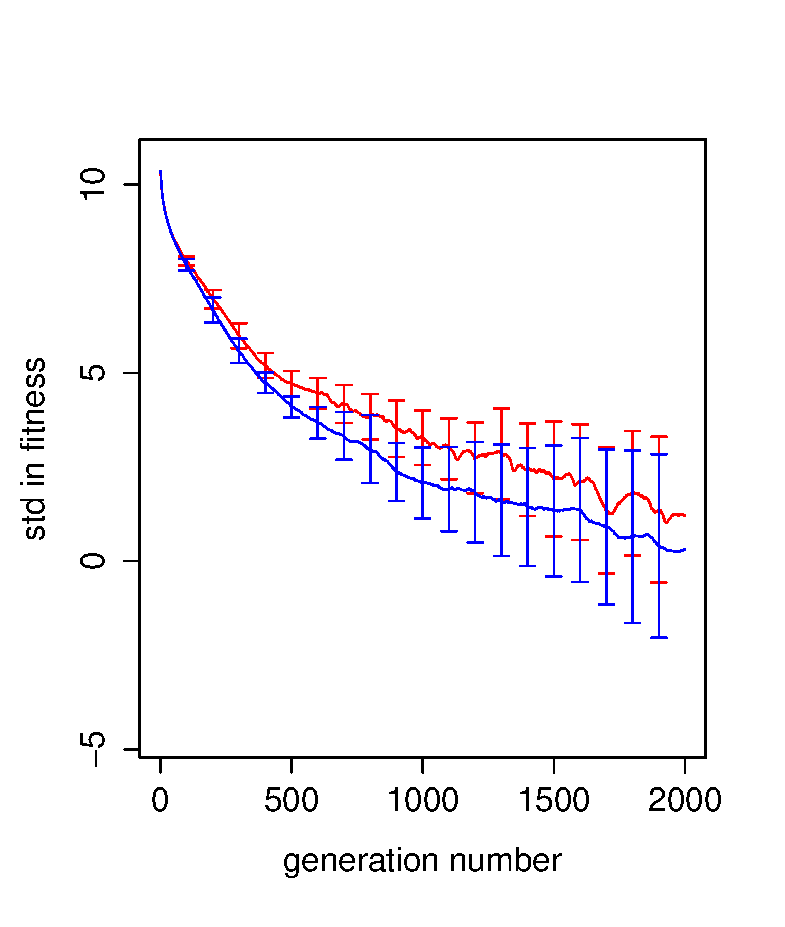
\includegraphics[clip, width=4.0cm]{P30fitD100.eps}
          \hspace{1.2cm} [14] P=30, D=100
        \end{center}
      \end{minipage}

      % 3
      \begin{minipage}{0.33\hsize}
        \begin{center}
          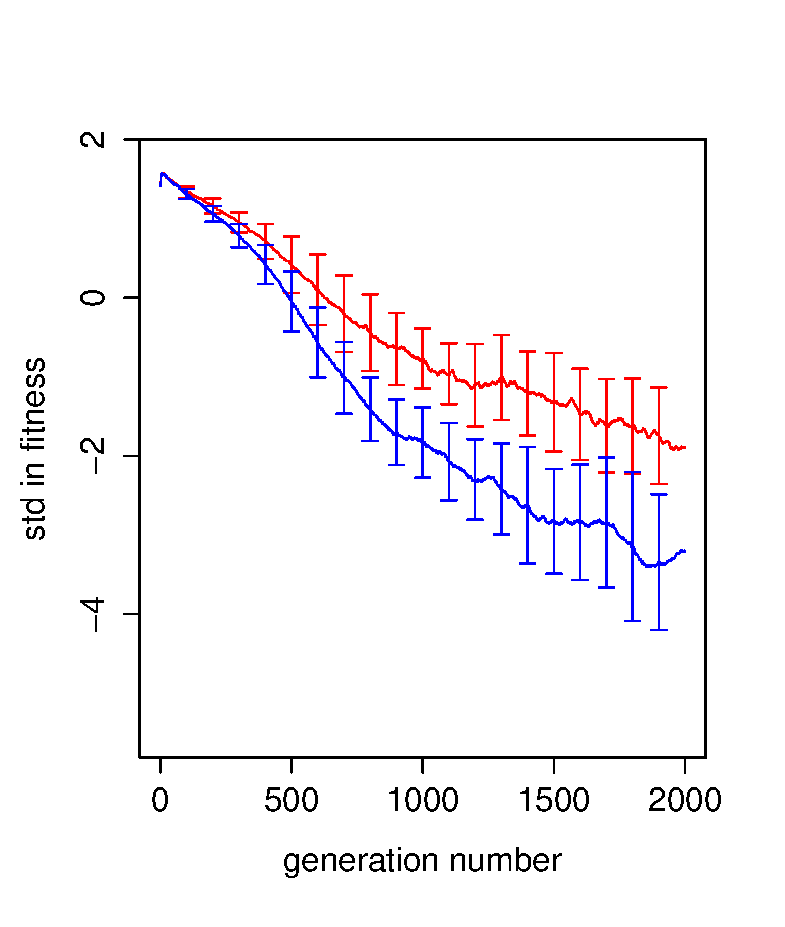
\includegraphics[clip, width=4.0cm]{P50fitD100.eps}
          \hspace{1.2cm} [15] P=50, D=100
        \end{center}
      \end{minipage}
    \end{tabular}
    \label{fig:lena}
  \end{center}
\end{figure}

\section{考察}
結果から,アーカイブがDEに与える多様性の維持はその問題設定における集団数$P$,次元数$D$が大きな影響を与えていることが分かった.集団数$P$が少なく,次元数$D$が大きいほど,アーカイブによって集団が多様性を維持したまま探索を続ける事ができる.これは,集団数$P$が少なく,次元数$D$が大きい時ほど,多様性維持がDEの探索において難しくなっていることが原因と考えられる.そのためアーカイブによる多様性維持が探索に与える影響が大きく現れている.
また今回の実験によって,確かにアーカイブを使用することで,使用しないときに比べて,集団が多様性をより維持しながら探索を続けることができることが分かった.

\chapter{アーカイブ改善の提案}
\section{提案手法:アーカイブサイズの廃止}
既存手法では,アーカイブのサイズは集団Pと同じサイズだけとり,超過分だけランダムにアーカイブから取りのぞく.このサイズが小さいと,解更新が停滞している場合,すぐに探索の近傍の個体でアーカイブが一杯になり,アーカイブで保持される個体の多様性が失われる.
現集団中の個体の各変数$j(j = 1,...,D)$の下限上限値を$[x_{min,j},x_{max,j}]^D$とする.
$alpha(>0)$である時,各世代の終了時に,アーカイブ内の全ての個体について,$[alpha *x_{min,j},alpha*x_{max,j}]^D$の範囲に全ての変数値が収まっていれば残し,そうでなければ削除する.
こうすることで,アーカイブのサイズがなくても,アーカイブに探索状況にあった多様な個体を保持できるのではと考えられる.
\section{実験設定}
ここでは突然変異戦略をcurrent-to-$p$best/bin/1及びパラメタを$F=0.5,CR=0.5$としたDEと,$alpha = (0.5, 1.0, 1.5, 2.0)$とした提案手法によるアーカイブを用いた,DEとで比較実験を行う.
評価実験にはBlack-Box Optimization Benchmarking at CEC'2015 (CEC-BBOB)の15個のベンチマーク関数を用いた.
全てのテスト関数において実行可能領域は$[-100,100]^D$である.また,探索中に得られた最良解と最適解との誤差が$10^{-8}$以下になった場合は,誤差値は0となる.ベンチマークの詳細については \cite{CEC2015} を参考にしていただきたい.
全てのテスト関数において次元数は$D=30$とし,1試行あたりの最大評価回数はD*10,000とした.試行回数は51回とし,この評価回数の平均値がどれほど高い精度の解であるかをもとに手法を評価する.また,有意水準0.05のWilcoxonの順位和検定を行った.


\section{実験結果}
\begin{table}[!tbp]
\footnotesize
\caption{提案手法と通常のDEの比較実験\label{ref-tb-values}} 
\begin{center}
\begin{tabular}{lrrrrr}
\hline\hline
\multicolumn{1}{l}{F}&\multicolumn{1}{c}{DE}&\multicolumn{1}{c}{DE}&\multicolumn{1}{c}{DE}&\multicolumn{1}{c}{DE}&\multicolumn{1}{c}{DE}\tabularnewline
&&\multicolumn{1}{c}{{\scriptsize alpha=(0.5)}}&\multicolumn{1}{c}{{\scriptsize alpha=(1.0)}}&\multicolumn{1}{c}{{\scriptsize alpha=(1.5)}}&\multicolumn{1}{c}{{\scriptsize alpha=(2.0)}}\tabularnewline
\hline
F1&$  55239682.383037$&$  117806536.459537$&$  123072395.547988$&$  123072395.547988$&$  107290052.452337$\tabularnewline
F2&$8529387307.018302$&$21471514156.285667$&$23288140436.411297$&$23288140436.411297$&$17104772991.747034$\tabularnewline
F3&$        20.850508$&$         20.883508$&$         20.884259$&$         20.884259$&$         20.873797$\tabularnewline
F4&$        96.140511$&$        110.058580$&$        102.324971$&$        102.324971$&$        102.683287$\tabularnewline
F5&$      2926.715271$&$       4480.793801$&$       4177.913026$&$       4177.913026$&$       4109.622982$\tabularnewline
F6&$    828727.133643$&$    2258704.772162$&$    1529747.414652$&$    1529747.414652$&$    1203940.957646$\tabularnewline
F7&$        40.785985$&$         94.626798$&$         90.005009$&$         90.005009$&$         64.558550$\tabularnewline
F8&$     93361.366973$&$     194313.951017$&$     260790.929820$&$     260790.929820$&$     159957.113523$\tabularnewline
F9&$       190.279114$&$        197.450897$&$        203.848363$&$        203.848363$&$        180.753619$\tabularnewline
F10&$   1325907.434102$&$    3480984.679354$&$    1533752.326741$&$    1533752.326741$&$    2124097.256893$\tabularnewline
F11&$       788.238449$&$        876.541485$&$        868.197686$&$        868.197686$&$        784.694925$\tabularnewline
F12&$       136.489411$&$        147.452971$&$        149.669454$&$        149.669454$&$        137.700912$\tabularnewline
F13&$       128.524648$&$        130.180770$&$        128.930424$&$        128.930424$&$        128.430373$\tabularnewline
F14&$     46682.002790$&$      53021.508935$&$      52068.379721$&$      52068.379721$&$      45561.385971$\tabularnewline
F15&$       605.813984$&$       3020.140593$&$       2453.868306$&$       2453.868306$&$       1340.193881$\tabularnewline
\hline
\end{tabular}\end{center}

\end{table}


\section{考察}

\chapter{終わりに}
\section{まとめ}
\section{謝辞}


%-----------------------------参考文献記述エリア---------------------------%
\begin{thebibliography}{10}
  \bibitem{Storn}R.Storn and K. Price. Differential evolution - a simple and efficient heuristic for global optimization over continuous spaces. Journal of Global Optimization, 11(4):341-359, 1997
  \bibitem{ExDE}K.V.Price, R, M.Storn and J.A. Lampinen.Differential Evolution - A Practical Approach to Global Opticization. Springer, Berlin Heidelberg, 2005.
  \bibitem{JADE}J. Zhang and A. C. Sanderson: JADE: Adaptive DifferentialEvolution With Optional External Archive,IEEE Tran. Evol.Comput.,13–5, 945/958 (2009)
  \bibitem{SHADE}R. Tanabe and A. Fukunaga: Success-History Based Param-eter Adaptation for Differential Evolution,Proceedings of the2013 IEEE Congress on Evolutionary Computation, 71/78(2013)
  \bibitem{CEC2015}Q. Chen, B. Liu,  Q. Zhang, J. J. Liang, P. N. Suganthan, B. Y. Qu, "Problem Definition and Evaluation Criteria for CEC 2015 Special Session and Competition on Bound Constrained Single-Objective Computationally Expensive Numerical Optimization", Technical Report, Computational Intelligence Laboratory, Zhengzhou University, Zhengzhou, China  and  Technical Report, Nanyang Technological University, Singapore, Nov 2014.

\end{thebibliography}
%---------------------------------必須エリア-------------------------------%
\end{document}


%----------------------------ファイルはここまで----------------------------%
